\documentclass{article}
\usepackage{style-notes}
\usepackage{hyperref}					% setup internal and external links
\hypersetup{							% set up hyperlinks (used for toc here)
   hidelinks,								% hide links (don't change appearance of text that is clickable)
   linktoc=all    								% make toc clickable (all levels)
}

\title{MATH 321: Mathematical Statistics\\ Notes}
\author{Colton Gearhart}
\date{\today}							

\begin{document}
\setcounter{secnumdepth}{0}		% trick to get unnumbered sections in table of contents
\maketitle
\dosecttoc
\tableofcontents
\newpage

%-------------------------------------------------------------------------
\section{Test 1}
%-------------------------------------------------------------------------

\secttoc

%----------------------------
\subsection{Lecture 14 -- Bivariate Distributions}
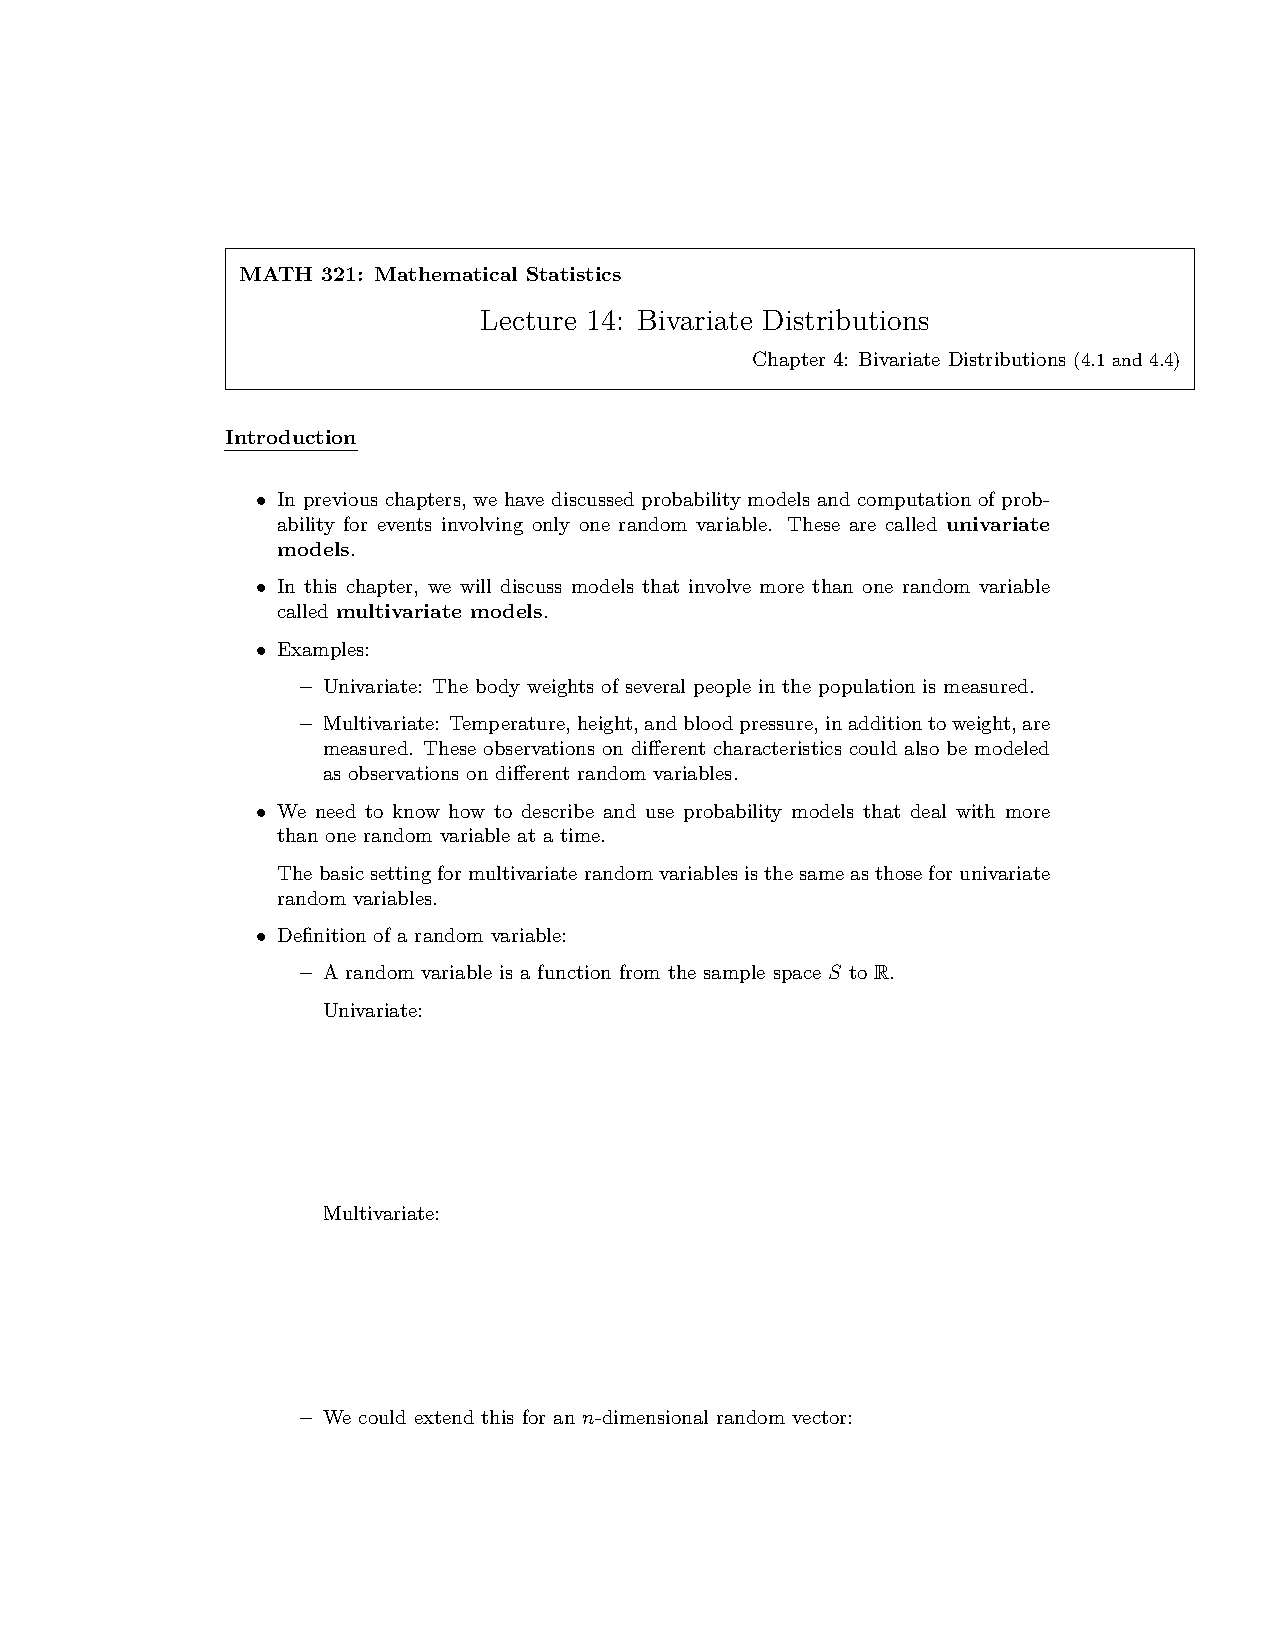
\includepdf[pages=-]{lecture-14.pdf}\newpage
%----------------------------
%
%%----------------------------
%\subsection{Lecture 1 -- XXX}
%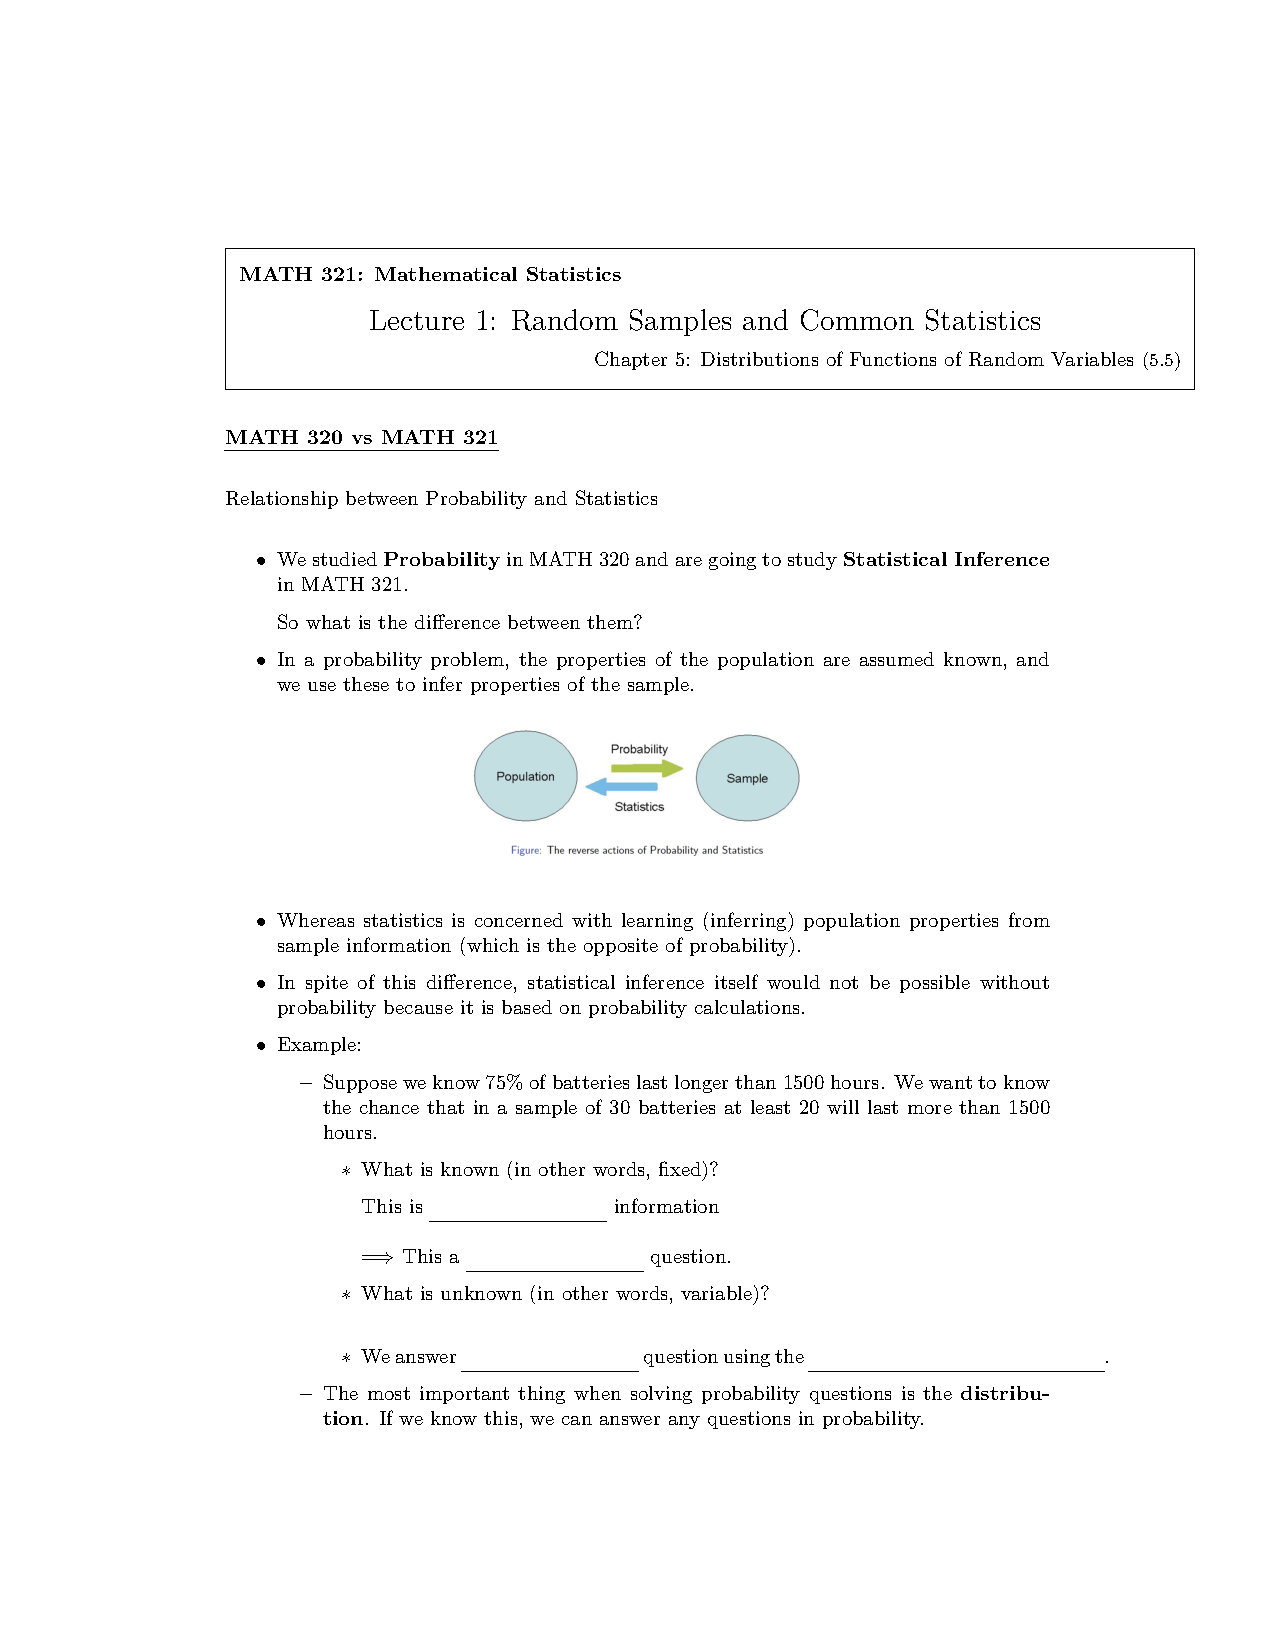
\includepdf[pages=-]{lecture-1.pdf}\newpage
%%----------------------------
%
%%----------------------------
%\subsection{Lecture 2 -- XXX}
%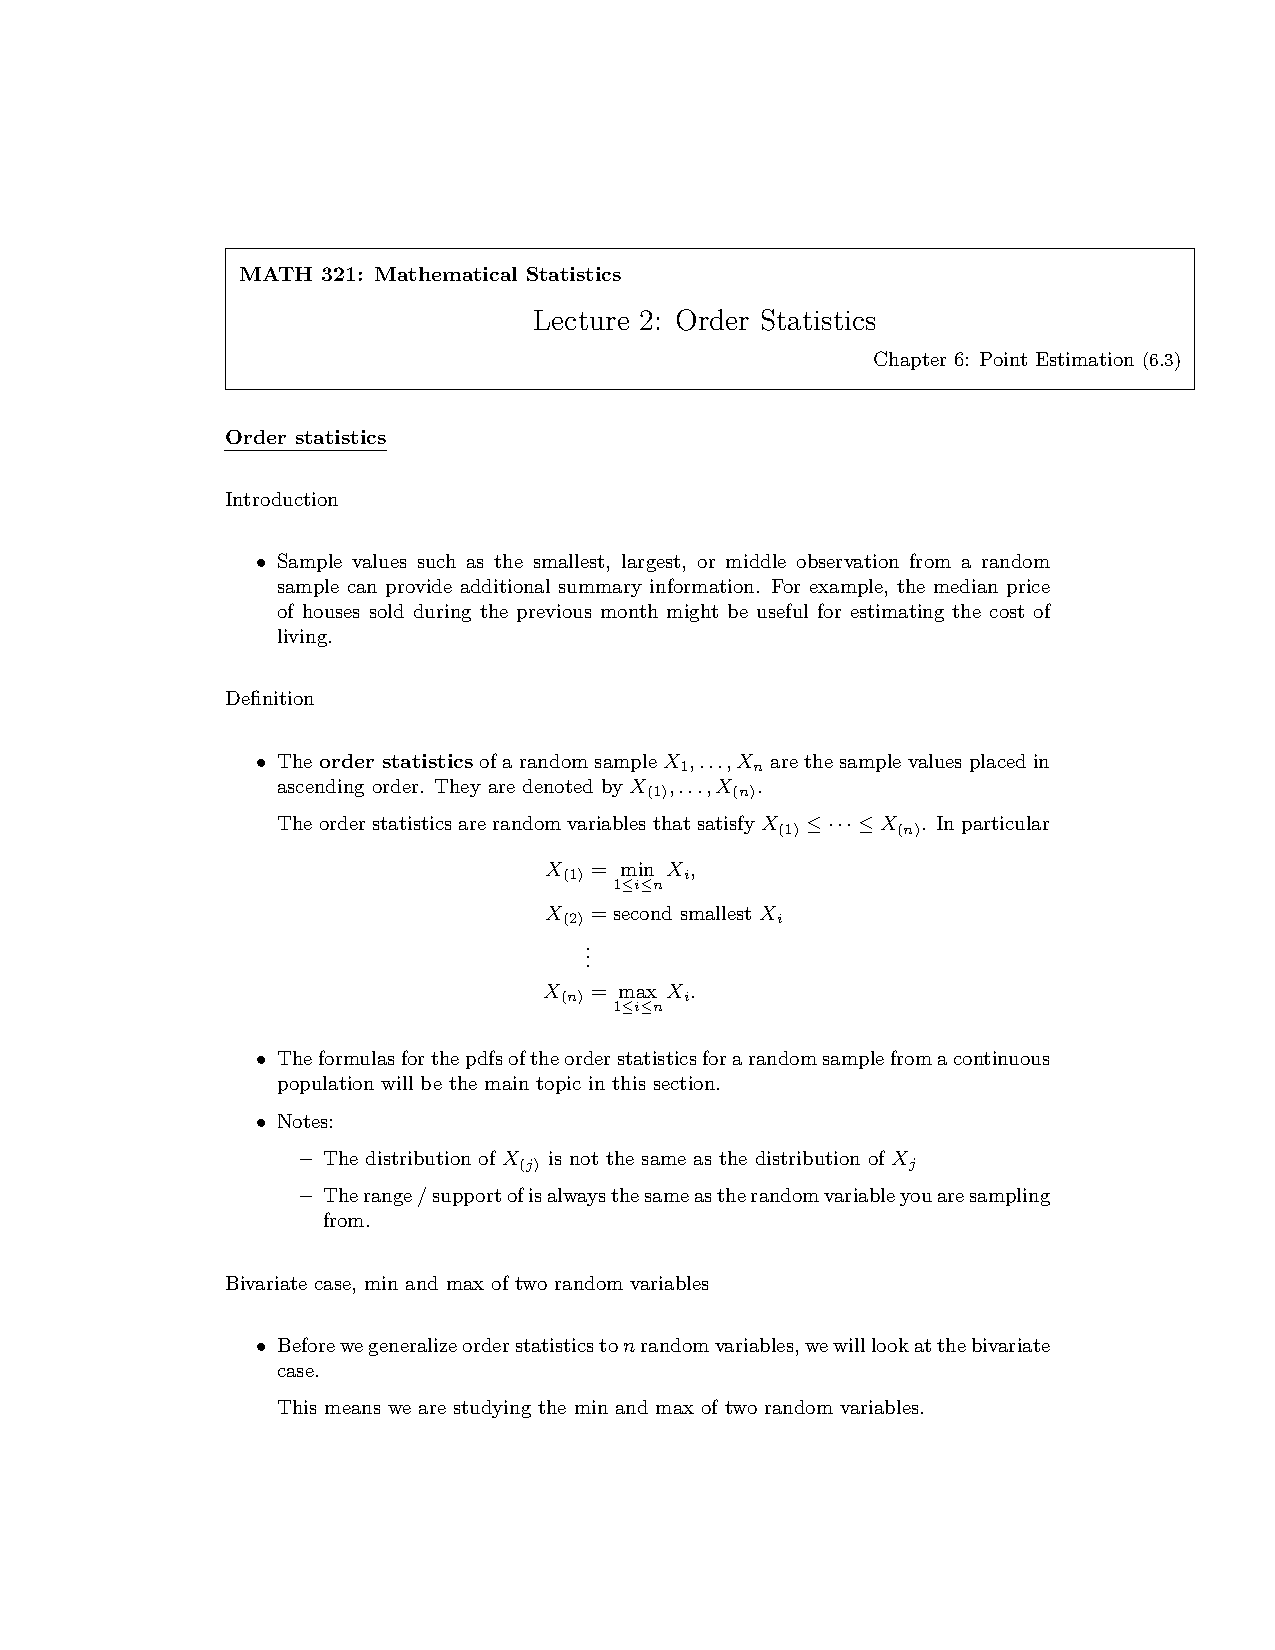
\includepdf[pages=-]{lecture-2.pdf}\newpage
%%----------------------------
%
%%----------------------------
%\subsection{Lecture 3 -- XXX}
%\includepdf[pages=-]{lecture-3.pdf}\newpage
%%----------------------------
%
%%----------------------------
%\subsection{Lecture 4 -- XXX}
%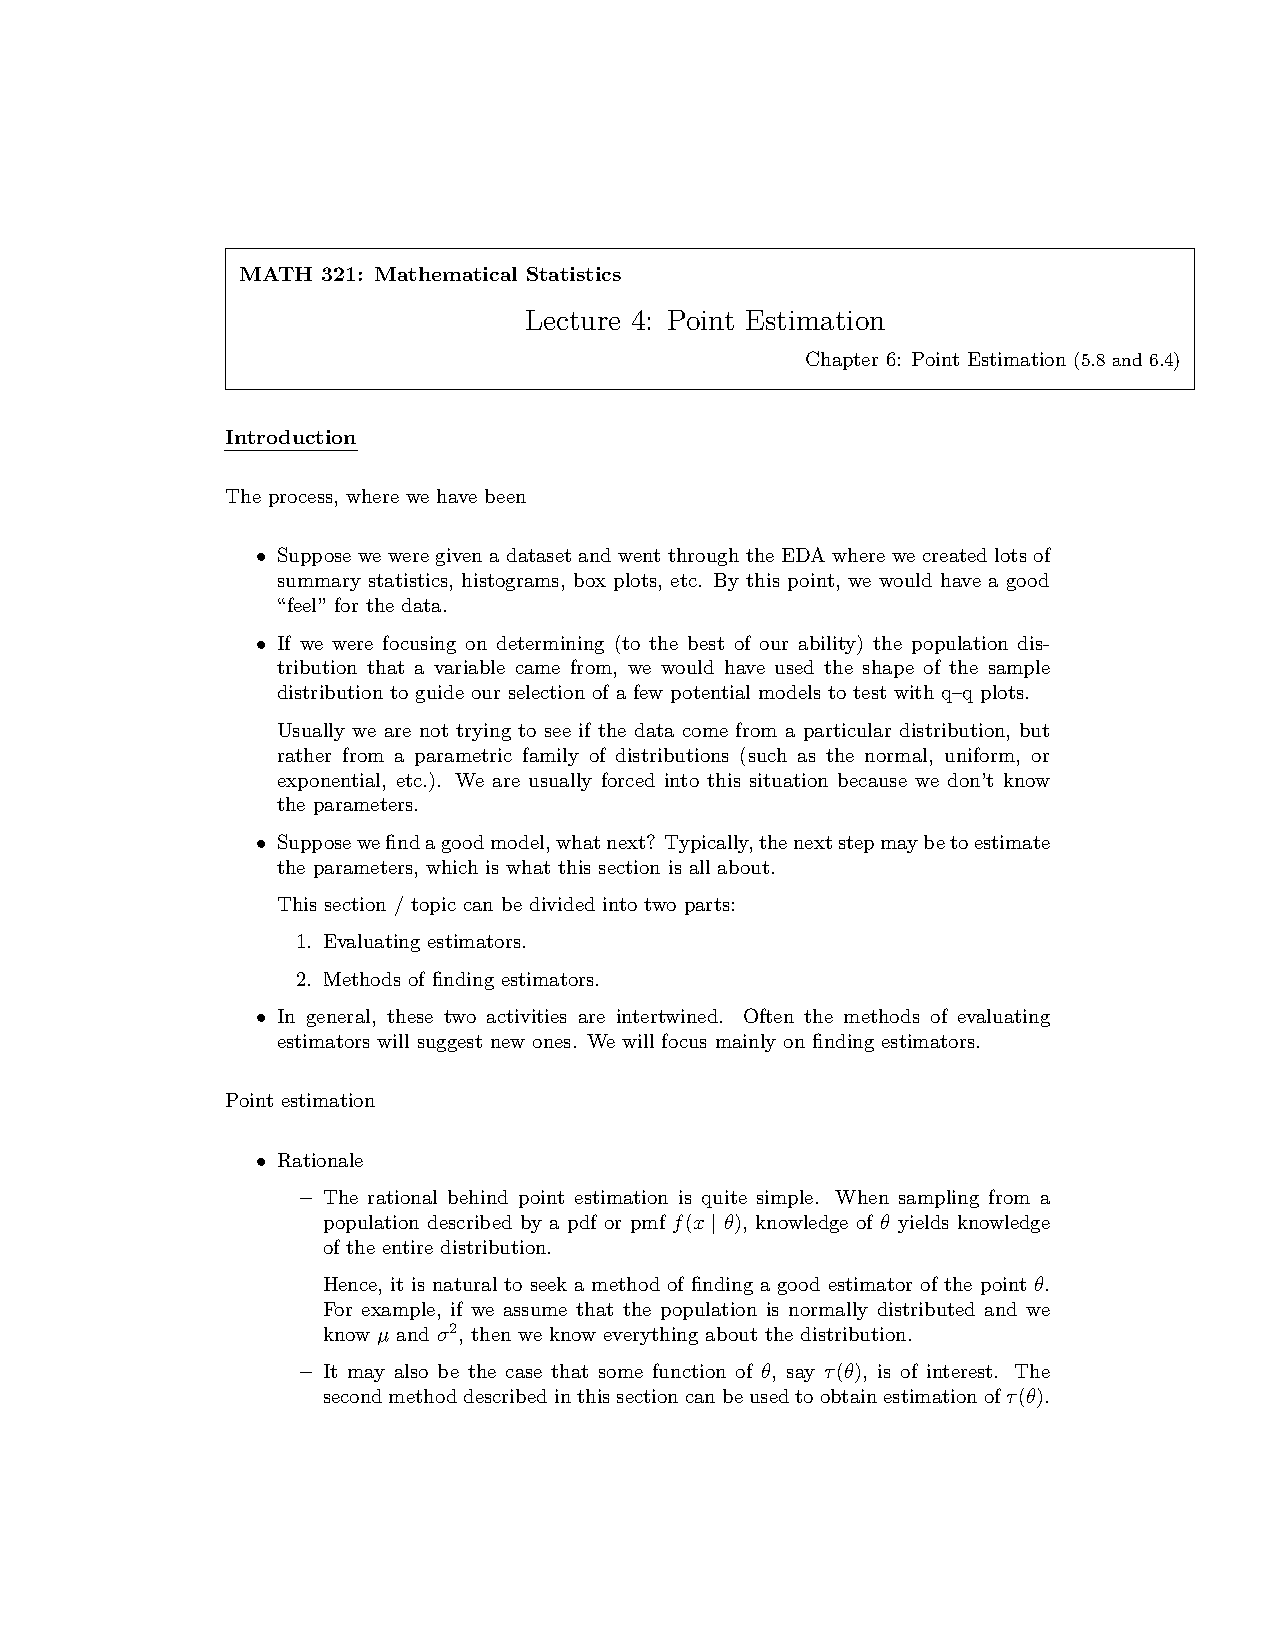
\includepdf[pages=-]{lecture-4.pdf}\newpage
%%----------------------------
%
%%----------------------------
%\subsection{Lecture 5 -- XXX}
%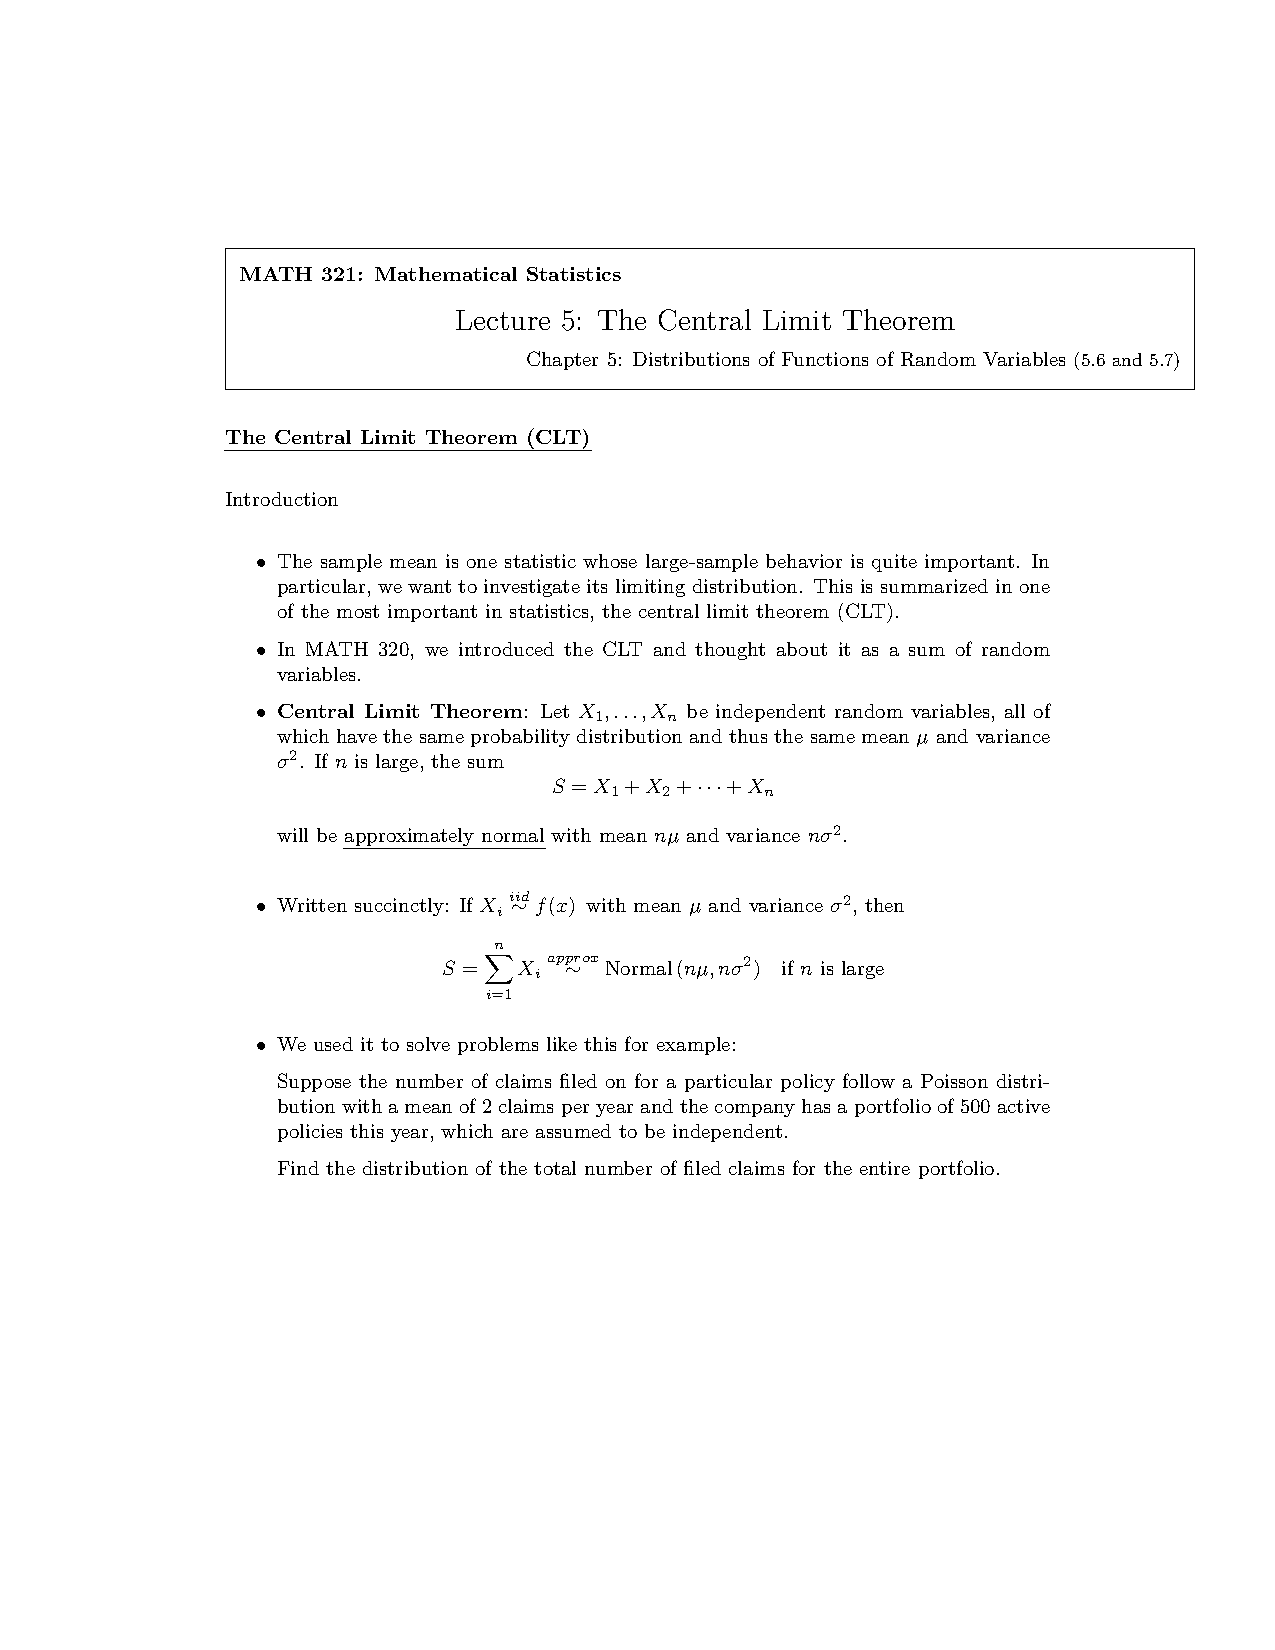
\includepdf[pages=-]{lecture-5.pdf}\newpage
%%----------------------------
%
%%----------------------------
%\subsection{Lecture 6 -- XXX}
%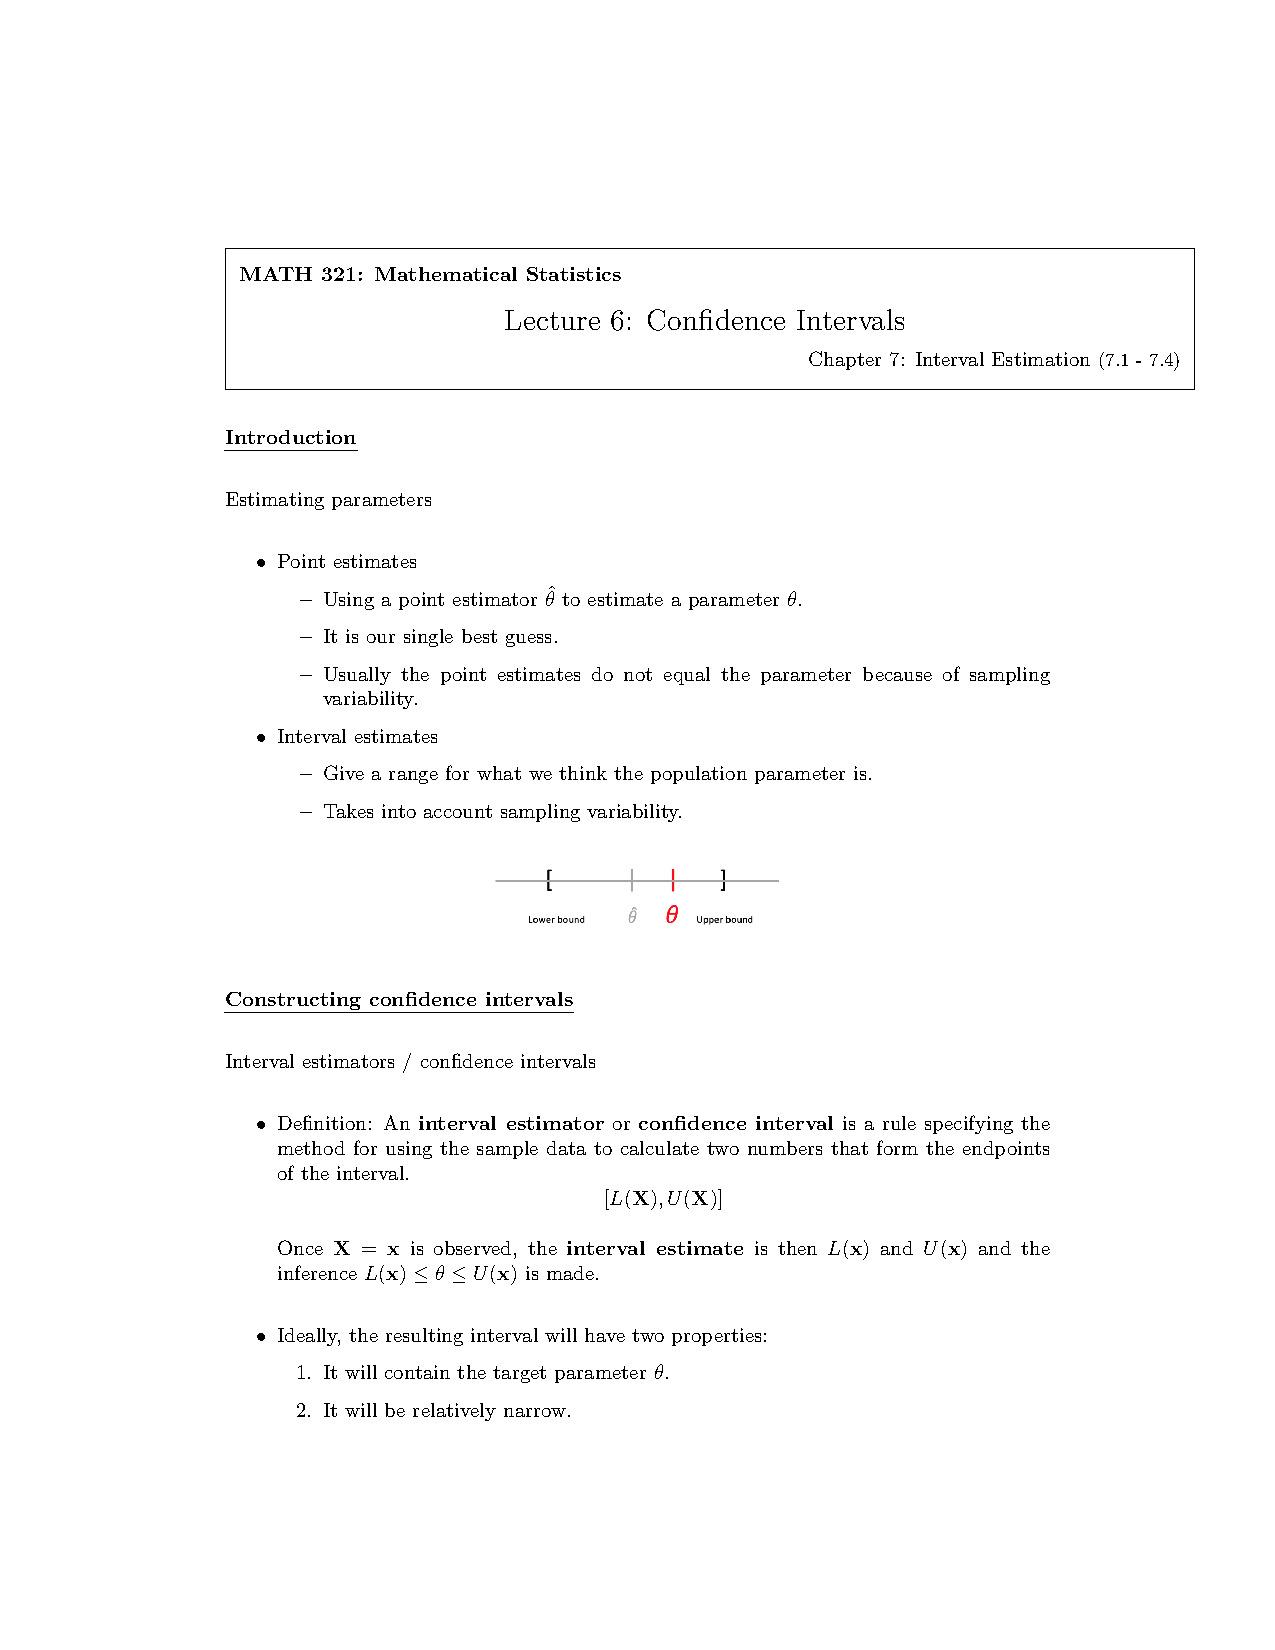
\includepdf[pages=-]{lecture-6.pdf}\newpage
%%----------------------------
%
%%-------------------------------------------------------------------------
%\section{Test 2}
%%-------------------------------------------------------------------------
%
%\secttoc
%
%%----------------------------
%\subsection{Lecture 7 -- XXX}
%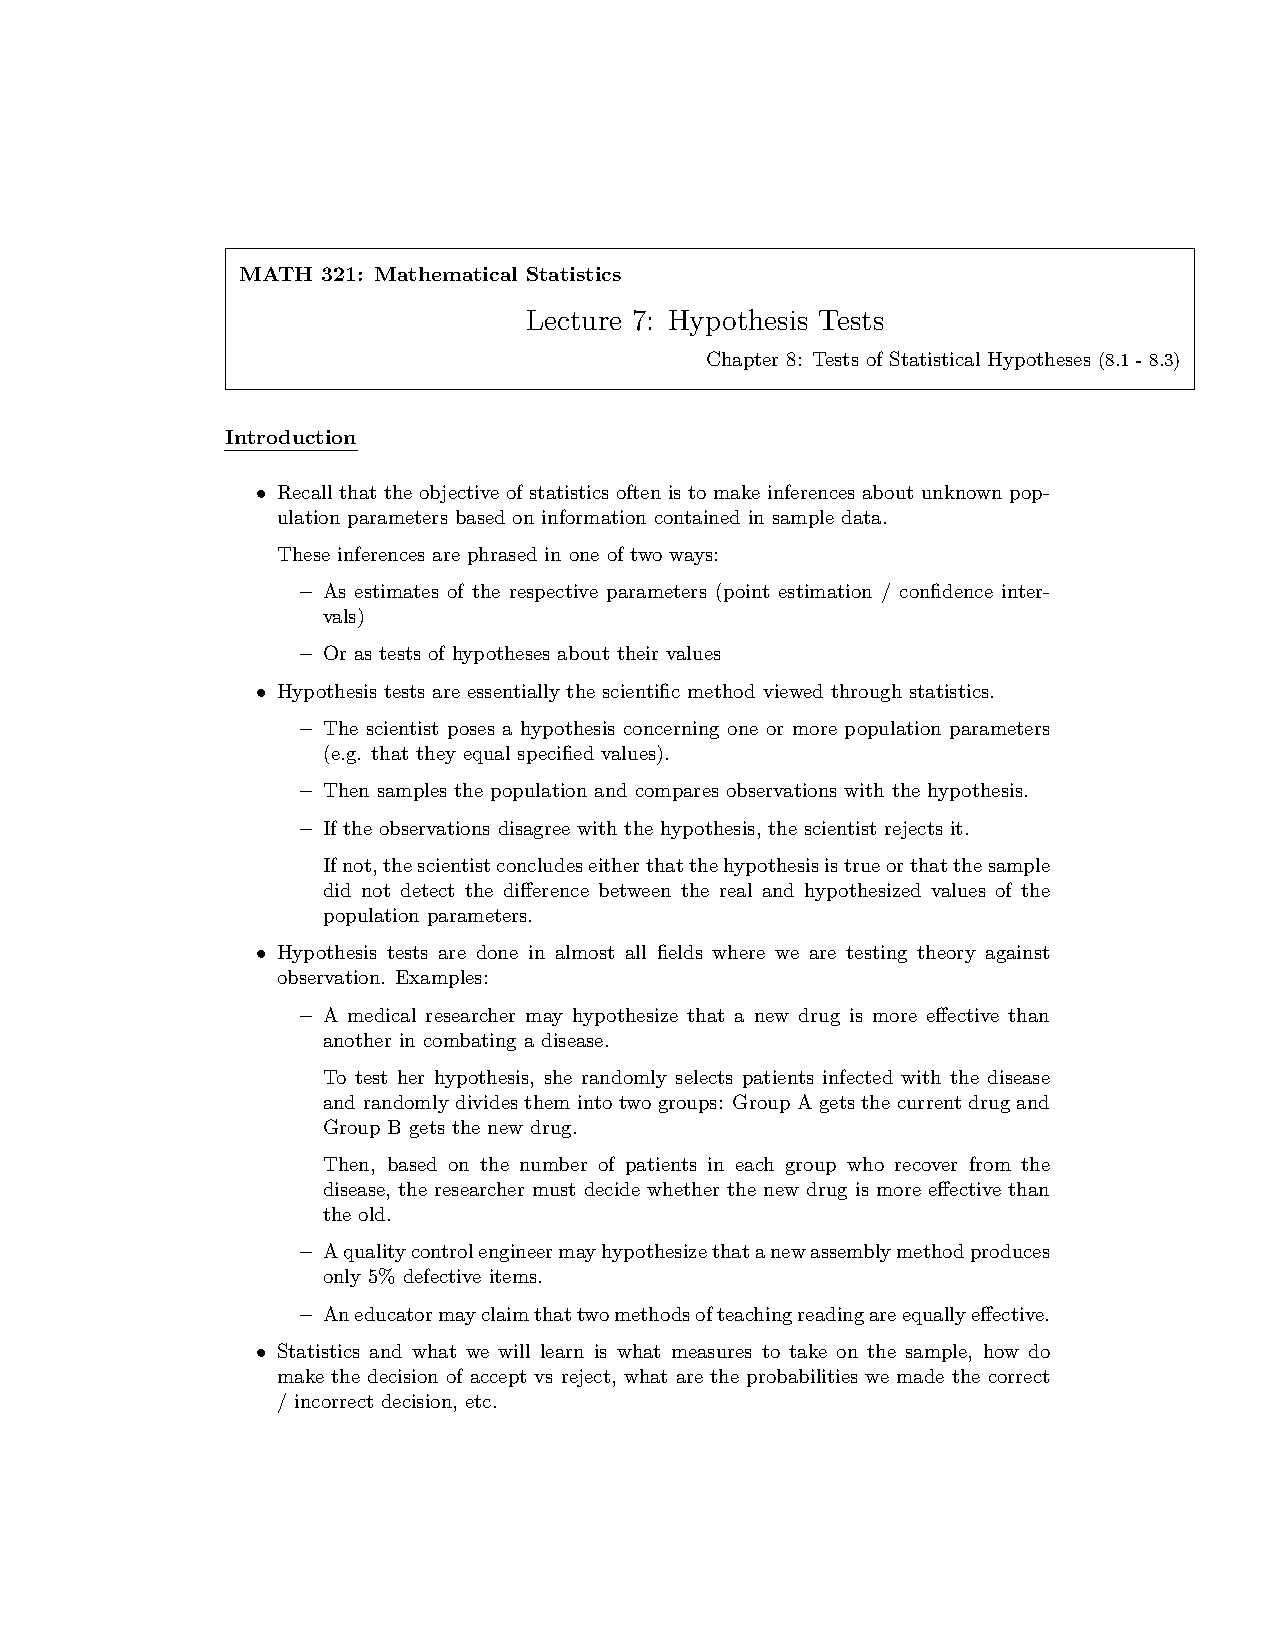
\includepdf[pages=-]{lecture-7.pdf}\newpage
%%----------------------------
%
%%----------------------------
%\subsection{Lecture 8 -- XXX}
%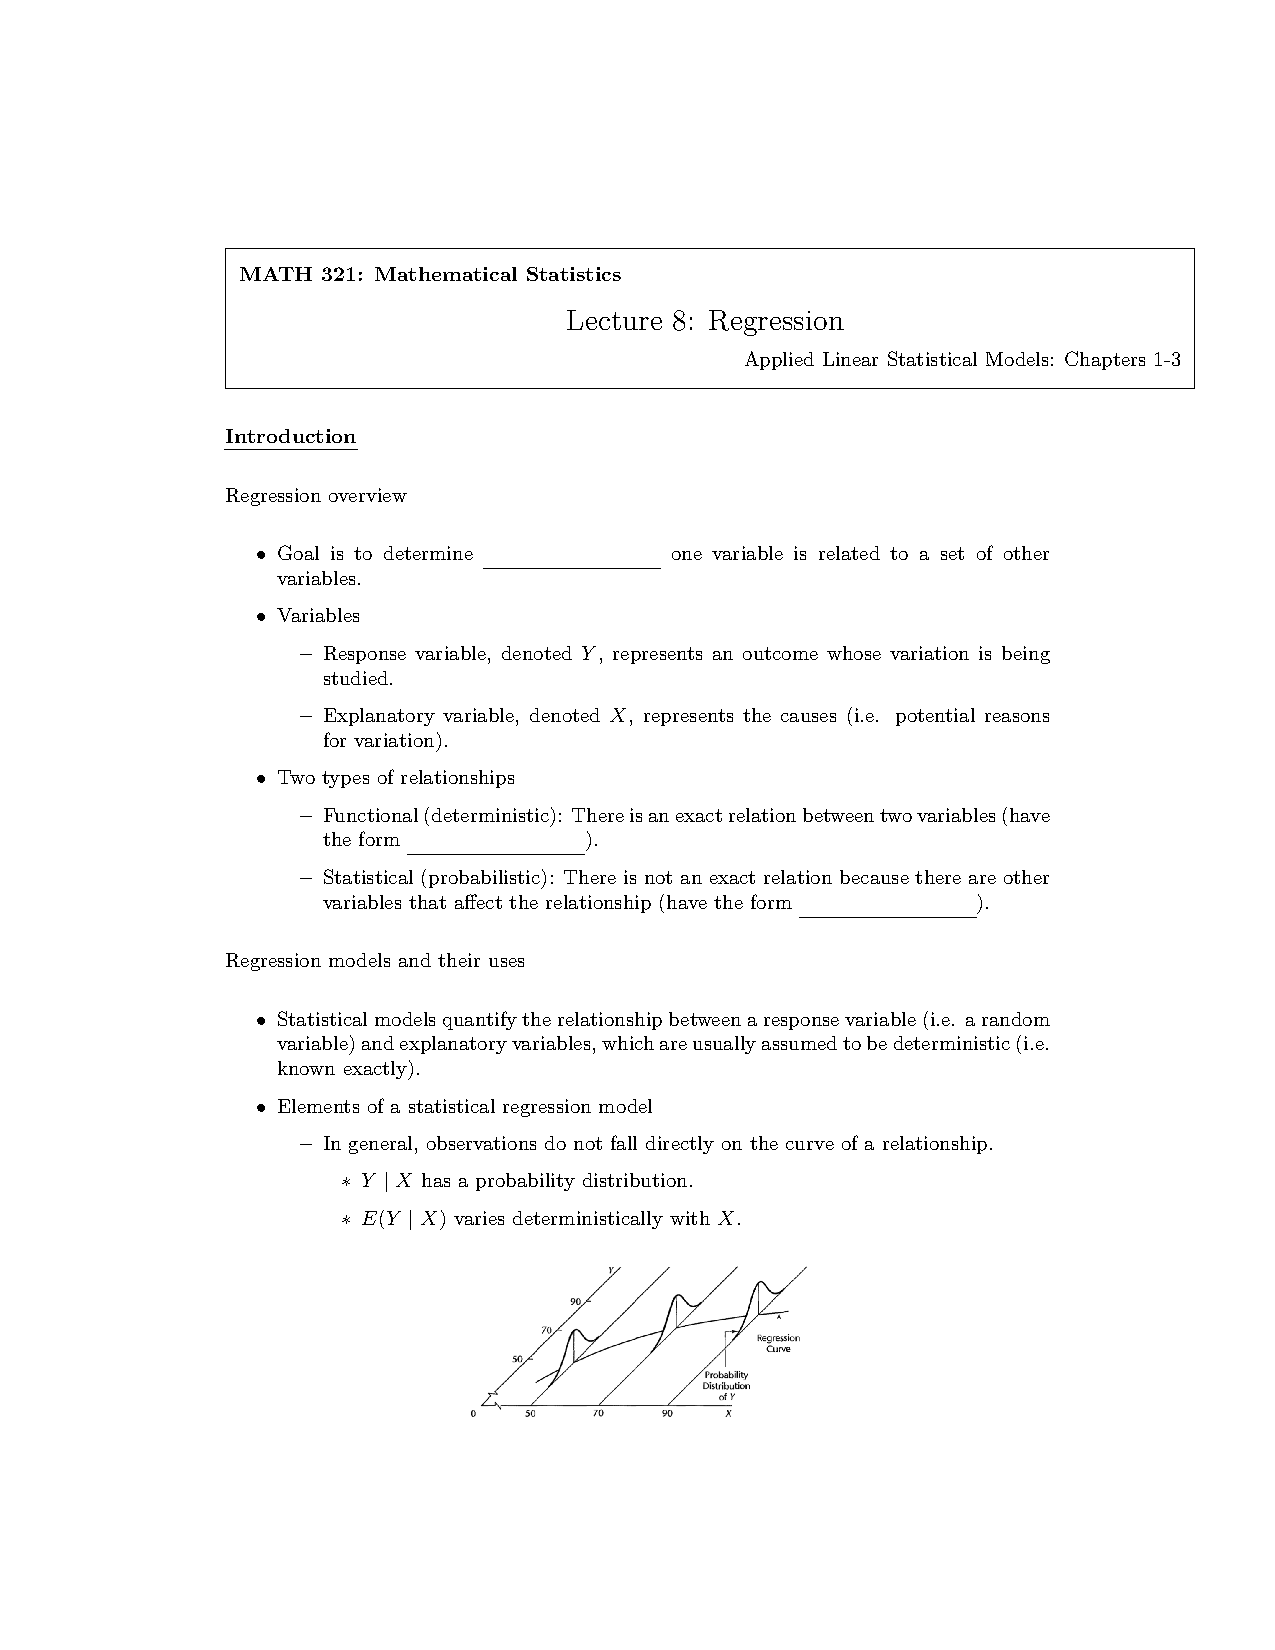
\includepdf[pages=-]{lecture-8.pdf}\newpage
%%----------------------------
%
%%----------------------------
%\subsection{Lecture 9 -- XXX}
%\includepdf[pages=-]{lecture-9.pdf}\newpage
%%----------------------------
%
%%-------------------------------------------------------------------------
%\section{Test 3}
%%-------------------------------------------------------------------------
%
%\secttoc
%
%%----------------------------
%\subsection{Lecture 10 -- XXX}
%\includepdf[pages=-]{lecture-10.pdf}\newpage
%%----------------------------
%
%%----------------------------
%\subsection{Lecture 11 -- XXX}
%\includepdf[pages=-]{lecture-11.pdf}\newpage
%%----------------------------
%
%%----------------------------
%\subsection{Lecture 12 -- XXX}
%\includepdf[pages=-]{lecture-12.pdf}\newpage
%%----------------------------
%
%%-------------------------------------------------------------------------
%\section{After Test 3}
%%-------------------------------------------------------------------------
%
%\secttoc
%
%%----------------------------
%\subsection{Lecture 13 -- XXX}
%\includepdf[pages=-]{lecture-13.pdf}\newpage
%%----------------------------


\end{document}